\section{UML}
Mas información para cada uno de estos diagramas en el apunte de Análisis de la Información. Acá solo se dejan breves descripciones.
\subsection*{Diagramas de actividad}
Para representar dinámicas del negocio, donde el tiempo va transcurriendo de arriba hacia abajo. Nos dan pie a los casos de uso.

\subsection*{Diagrama de Casos de uso}
Cada una de las actividades esta representada acá. Puede ocurrir que después algún caso de uso se parta en varios mas, que se representarían en otro diagrama. 

\subsection*{Diagrama de estados}
Se realizan para algunos de los objetos creados para indicar el paso de estados. No se indica que hace que pase de estados, sino los cambios posibles.

\subsection*{Diagrama de paquetes}
\begin{itemize}
\item Los negocios por lo general tienen múltiples contextos, que analizados con las herramientas empiezan a tomar forma en paquetes (parte de nuestros negocios). 
\item Permiten concentrar la dinámica de nuestro negocio desde el punto de vista del negocio.
\item Paquetes de un alto nivel, paquetes de nivel intermedio, y después de mas bajo nivel.
\item Los paquetes se asocian con componentes, que a su vez estan asociados a nodos.
\item Son muy intuitivos, pero poco rigurosos. Hay que tener en cuenta la inversión en la cadena de dependencia (principio). Esto no es tenido en cuenta en los siguientes gráficos de paquetes.
\end{itemize}


\begin{figure}[!htb]
    \centering
    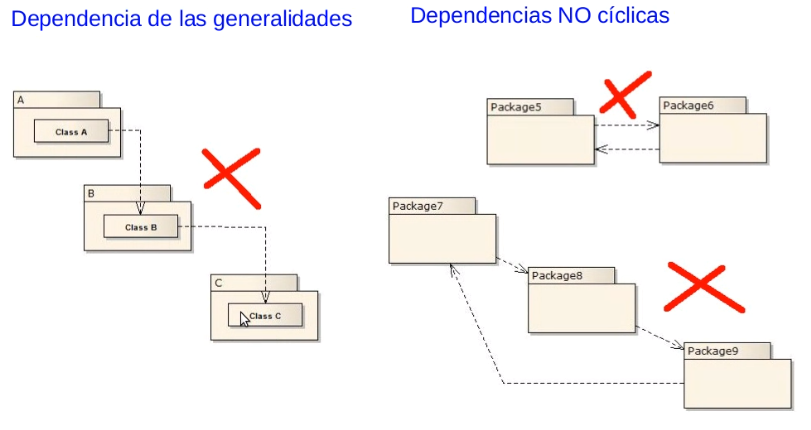
\includegraphics[width=0.6\textwidth]{img/paq.PNG}
\end{figure}

Para que nuestro diseño goce de esto, el nivel superior debe estar compuesto por abstracciones/generalidades, y los niveles inferiores de cuestiones concretas que dependen de las generalidades. 

\begin{figure}[!htb]
    \centering
    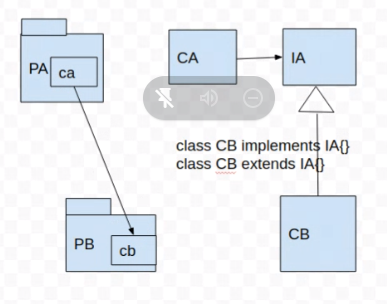
\includegraphics[width=0.8\textwidth]{img/paqbien.PNG}
\end{figure}

% imagen
% ca y ia dentro del paquete PA
Se cumple la inversión en la cadena de dependencia
Hay que hacer el gráfico de la derecha para cuestiones vinculadas al diseño. % cuestion para ser mas cuidadoso en uml

\subsection*{Otras cuestiones de UML mencionadas}
\begin{itemize}
\item Composición, no puede existir la clase A sin la clase B, seria incompatible. Corresponde a un Ensamble-Parte.
\item Agregación, puedo construir tipo A sin B. Se agrega un agregador de B. Cuando lo tenga, A no es dueño de B.\textit{ (Llevándolo a C++, A no seria el encargado de destruir a B, ya que no es dueño de B)}
\item De uso, asociación, solamente utiliza al objeto.
\end{itemize}

